\documentclass[border=4pt]{standalone}
\usepackage[T1]{fontenc}
\usepackage{helvet}
\renewcommand{\familydefault}{\sfdefault}
\usepackage{graphicx}
\usepackage{caption}
\usepackage{amsmath}
\captionsetup{font={sf,footnotesize},labelfont={sf,bf,footnotesize},justification=justified,singlelinecheck=false}
\begin{document}
\setcounter{figure}{13}
\begin{minipage}{7.20in}
\centering
\begin{figure}[htbp]
    \centering
    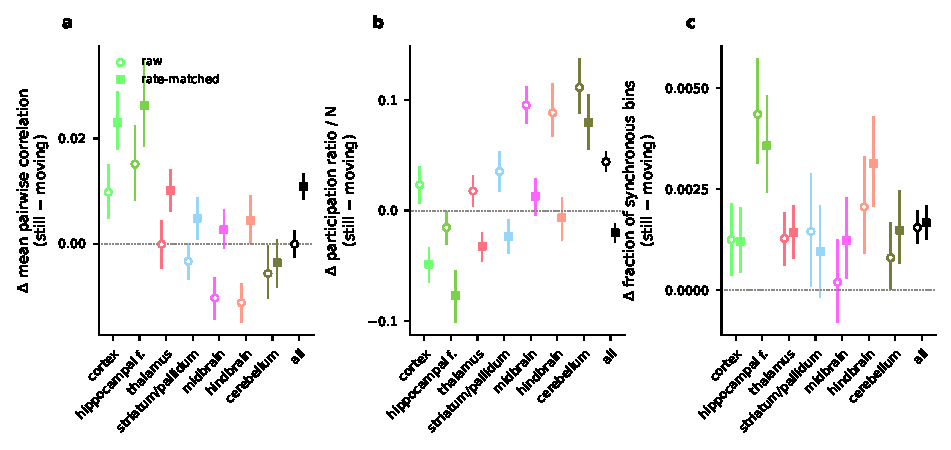
\includegraphics[width=\linewidth]{fig14_still_population_panels.pdf}
    \caption{In stillness, neurons within a region fluctuate together more (rate-matched), most clearly in cortex and hippocampus. \textbf{a} Mean pairwise spike-count correlation within a region (100\,ms bins, equal numbers of still and moving bins), still minus moving, per region and probe averaged within mouse; mean over mice and bootstrap 95\% CI. Open: raw counts; filled: each neuron's counts in its higher-rate state binomially thinned to its rate in the other state. Rate-matched, 82\% of 129 mice have higher correlation in stillness (cortex 91\%). \textbf{b} Participation ratio of the correlation matrix divided by the number of neurons (dimensionality). The raw increase in stillness disappears after rate matching. \textbf{c} Fraction of 100\,ms bins in which the summed population count exceeds its within-state mean by 3 SD (synchronous events).}
    \label{fig:population}
\end{figure}
\end{minipage}
\end{document}
